\section{Μαθηματικό Υπόβαθρο}
\label{chapBackground}

\subsection{Πλέγματα}

\begin{definition}:
 \textbf{ Πλέγμα } (ή δικτυωτό) ονομάζουμε ένα σύνολο σημείων $L$ του $n$-διάστατου χώρου $	\mathbb{R}^n$, τα οποία προκύπτουν ως ακέραιος γραμμικός συνδυασμός μιας σειράς γραμμικώς ανεξάρτητων διανυσμάτων $\{{ \bm b_i}\}_{i=1}^k, (k \leq n)$.
 
 $$ L(\bm b_1, ...,\bm b_n) = \bigg\{ \sum_{i=1}^{k} x_i \cdot \bm b_i, x_i \in \mathbb{Z}  \bigg\} = \bigg\{ \bm x \bm B, \bm x \in \mathbb{Z}^k \bigg\}$$

\end{definition}

Τα διανύσματα $ \{\bm b_i \}$ αποτελούν τις γραμμές του πίνακα Β, διάστασης $ k \times n $ και ονομάζονται βάση του πλέγματος. Λέμε ότι μία βάση παράγει ένα πλέγμα, αλλά επίσης ισχύει ότι ένα πλέγμα μπορεί να παράγεται, από παραπάνω από μία βάσεις. Σε κάθε περίπτωση όλες οι βάσεις ενός πλέγματος έχουν τον ίδιο αριθμό στοιχείων $ k $, που ονομάζεται τάξη (\lt rank). O αριθμός $ n $ των στοιχείων που απαρτίζουν κάθε διάνυσμα ονομάζεται διάσταση του πλέγματος. Αν $ n=k $ τότε το πλέγμα καλείται μέγιστης τάξης (\lt full rank lattice). Στην παρούσα πτυχιακή εργασία ασχολούμαστε με πλέγματα αυτής της κατηγορίας.

\begin{definition}:
 \textbf{Ορίζουσα} (\lt determinant) ενός πλέγματος $ L(\bm B) $ καλούμε την ποσότητα:
 
 $$ det(L(\bm B)) = \sqrt{det(\bm B^T \bm B)}$$
 
και στην ειδική περίπτωση των πλεγμάτων μέγιστης τάξης ισχύει:

$$ det(L(\bm B)) = | det(\bm B) | $$

Δηλαδή η ορίζουσα του πλέγματος ισούται με την απόλυτη τιμή της ορίζουσας του πίνακα βάσης αυτού. Ωστόσο, αξίζει να σημειωθεί ότι η ορίζουσα αυτή είναι ανεξάρτητη από την επιλογή της βάσης.
 
\end{definition}

Τέλος με τον όρο, \textbf{ελάχιστο} ενός δικτυωτού $ L $, αναφερόμαστε στη νόρμα του μικρότερου μη-μηδενικού διανύσματος και συμβολίζεται $ \lambda_1(L) $.

% $$ λ_1(L) = \inf \{ \| \bm x \| \}, \bm x \in L - \{0\} $$

$$ λ_1(L) = \inf \big\{ ||{\bf x}|| : {\bf x}\in L-\{{\bf 0} \} \big\} $$

\subsection{$n$-διάστατη Μπάλα}

Σε αυτή την παράγραφο παραθέτουμε τα βασικά μεγέθη που χαρακτηρίζουν μια $n-$διάστατη μπάλα του $ \mathbb{R}^n $. Πρόκειται για μια μαθηματική έννοια, που θα μας βοηθήσει στη συνέχεια να προχωρήσουμε την ανάλυσή μας.

%  αναφερόμαστε στον τοπολογικό χώρο που στα μαθηματικά αποκαλούμε \textbf{μπάλα}. Κρίθηκε σημαντικό να

\begin{definition} : Ως \textbf{$n-$διάστατη Μπάλα}, ορίζουμε το σύνολο των σημείων που περικλείονται από μία σφαίρα. Δηλαδή μια κλειστή μπάλα ακτίνας $ R > 0 $ με κέντρο την αρχή των αξόνων $ \bm 0 $ είναι το σύνολο:

$$ Β_n(R) = \{\bm x \in \mathbb{R}^n : \| \bm x \| \leq R  \} $$

\end{definition}

Εν γένει ο όγκος της $n-$διάστατης μπάλας και η επιφάνεια της $(n-1)-$διάστατης σφαίρας που την περικλείει είναι αναλογικά της ακτίνας $ R $, εις τη διάσταση του χώρου. Συνηθίζουμε να γράφουμε $ V_n(R) = V_nR^n $ και $ S_n(R) = S_nR^n $, όπου $ V_n = V_n(1) $, $ S_n = S_n(1) $, δηλαδή ο όγκος και το εμβαδόν της μοναδιαίας n-διάστατης μπάλας/σφαίρας, αντίστοιχα. Στη συνέχεια δίνουμε τους κλειστούς τύπους αυτών των μεγεθών \cite{ball}.

Όγκος $n-$διάστατης μπάλας:

\begin{equation} \label{volume}
    V_n(R) = \dfrac{\pi^{n/2}}{\Gamma(\frac{n}{2}+1)}R^n
\end{equation}

Επιφάνεια περιβάλλουσας $n-$διάστατης σφαίρας:

\begin{equation} \label{surface}
   S_n(R) = \dfrac{2\pi^{\frac{n+1}{2}}}{\Gamma(\frac{n+1}{2})}R^n
\end{equation}

με τη συνάρτηση γάμμα να ορίζεται ως:

$$ Γ(s) = \int_{0}^{\infty} x^{s-1} e^{-x} dx, s > 0 $$


\subsection{Πρόβλημα του μικρότερου διανύσματος}

Τα κυριότερα προβλήματα που ανακύπτουν στα πλέγματα και στα οποία μπορεί να βασιστεί ένα κρυπτογραφικό σύστημα, είναι το πρόβλημα της εύρεσης του μικρότερου (SVP) καθώς και του εγγύτερου διανύσματος (CVP). Παρουσιάζουμε αναλυτικά αυτά τα προβλήματα στη συνέχεια. 

\begin{definition}:
 \textbf{Shortest Vector Problem (SVP)}: Δοθέντος ενός πλέγματος $ L $ τάξης $ n $, να βρεθεί το μικρότερο μη μηδενικό διάνυσμα $ \bm v $. Δηλαδή αναζητούμε το διάνυσμα $ \bm v $ ώστε: 
 % καθώς και μιας νόρμας $ Ν $ 
 $$ \| \bm v \| = \lambda_1(L) $$
 
 με $ \lambda_1(L) $ συμβολίζουμε το μέτρο του ελάχιστου διανύσματος.
\end{definition}

Αποδεικνύεται ότι τέτοιο διάνυσμα υπάρχει και μάλιστα δεν εξαρτάται από την επιλογή της βάσης του πλέγματος. Ορίζουμε επίσης και την προσεγγιστική εκδοχή του συγκεκριμένου προβλήματος ($ SVP_{\gamma} $), όπου αναζητούμε όχι το μικρότερο πλέον, αλλά ένα διάνυσμα που δεν υπερβαίνει το μικρότερο κατά έναν πολλαπλασιαστικό παράγοντα γ, δηλ: 

$$ \| \bm v \| \leq \gamma \cdot \lambda_1(L),  \gamma \geq 1$$

Ο \lt Ajtai απέδειξε ότι το SVP είναι NP-hard υπό τυχαίες αναγωγές \cite{Ajtai}. Για την επίλυση του συγκεκριμένου προβλήματος, δύο οικογένειες αλγορίθμων είναι γνωστές. Οι αλγόριθμοι που βασίζονται σε απαρίθμηση (\lt enumeration algorithms) και οι αλγόριθμοι κοσκινίσματος (sieving algorithms). 

\subsection{Πρόβλημα του εγγύτερου διανύσματος}

\begin{definition}:
 \textbf{Closest Vector Problem (CVP)}: Δοθέντος ενός πλέγματος $ L $ τάξης $ n $, μιας απόστασης $ Μ $, καθώς και ενός διανύσματος στόχου $\bm t \in \mathbb{R}^n $, να βρεθεί το πλησιέστερο στο $\bm t $, διάνυσμα του πλέγματος $ L $.  Δηλαδή αναζητούμε το $\bm v_* \in L $ ώστε: 
 
 $$ Μ(\bm v_*- \bm t) = \min_{\bm v} M(\bm v-\bm t) $$
 
\end{definition}

Αντίστοιχα και με το προηγούμενο πρόβλημα, δίνουμε την προσεγγιστική εκδοχή $ CVP_{\gamma} $, όπου πλέον αναζητούμε ένα διάνυσμα $ v \in L $ ώστε: 

$$ Μ(\bm v_*-\bm t) \leq \gamma \cdot \min_{\bm v} M(\bm v- \bm t),  \gamma \geq 1$$ 

Το CVP είναι επίσης υπολογιστικά δυσεπίλυτο και ανήκει στην κλάση των NP-hard προβλημάτων. Τέλος συνηθέστερα στο CVP ως συνάρτηση απόστασης χρησιμοποιείται η Ευκλείδεια.  

\subsection{Θεώρημα του \lt Minkowski}

Από τους παραπάνω ορισμούς για το πρόβλημα του μικρότερου διανύσματος \lt SVP, γεννάται το ερώτημα, ποιο είναι αυτό το ελάχιστο μήκος του διανύσματος που αναζητούμε.
Η ακριβής εύρεση αυτού είναι μια εξαιρετικά δύσκολη υπόθεση. Σε αυτό έρχεται να μας βοηθήσει το θεώρημα Minkowski. 

\begin{theorem} (1ο Θεώρημα του Minkowski): Δοθέντος ενός πλέγματος διάστασης n, μιας ακτίνας $ R>0 $ και της μοναδιαίας n-διάστατης σφαίρας του $ \mathbb{R}^n $, της οποίας ο όγκος ικανοποιεί τη σχέση:

\begin{equation} \label{limitation}
    V_nR^n > det(L)
\end{equation}

υπάρχει διάνυσμα $\bm v \in L-\{\bm 0\} $ με: 

\begin{equation} \label{bound}
    \| \bm v \| \leq 2R
\end{equation}

\end{theorem}

Από τις εξισώσεις (\ref{limitation}) και (\ref{bound}) γίνεται φανερό πως μία $n$-διάστατη μπάλα με ακτίνα τουλάχιστον:

\begin{equation}
    R_o = 2 \bigg( \dfrac{\det{L}}{V_n} \bigg) ^{1/n} \numeq{\ref{volume}} 2 \dfrac{(\det{L})^{1/n} \Gamma(\frac{n}{2} + 1)^{1/n} }{\sqrt{\pi}} 
\end{equation}

περιέχει ένα μη μηδενικό διάνυσμα του L.

Το Θεώρημα Minkowski καταφέρνει λοιπόν με αυτόν τον τρόπο να συνδέσει την ορίζουσα του πλέγματος, det(L), με το μήκος του μικρότερου διανύσματος του L. 

\subsection{Ευρετική του \lt Gauss}

H ποσότητα που μόλις αναφέραμε προσεγγίζεται από την Ευρετική του Gauss:

\begin{definition}: Ορίζουμε ως \textbf{Gaussian Heuristic} τον θετικό πραγματικό αριθμό:

\begin{equation}
    GH(L) = \bigg( \dfrac{\det{L}}{V_n} \bigg) ^{1/n} \numeq{\ref{volume}}  \dfrac{(\det{L})^{1/n} \Gamma(\frac{n}{2} + 1)^{1/n} }{\sqrt{\pi}} \approx \sqrt{\dfrac{n}{\pi e}} (\det{L})^{1/n}
\end{equation}

\end{definition}

Αποδεικνύεται ότι μεταξύ του ελαχίστου ενός πλέγματος και της \lt Gaussian Ευρετικής ισχύει η σχέση: $$ λ_1(L) < 2GH(L) $$

\begin{definition} : (Ευρετική υπόθεση Gauss). Για τυχαίο ακέραιο πλέγμα $ L $ τάξης k και διάστασης n, θεωρούμε ότι: 

$$ \lambda_1(L) \approx GH(L) $$

\end{definition}

Η ευρετική του Gauss δεν ισχύει για όλα τα ακέραια πλέγματα, όμως ουσιαστικά πετυχαίνει να μειώσει στο μισό την ακτίνα μιας μπάλας με κέντρο την αρχή, προκειμένου εκείνη να περιέχει ένα μη μηδενικό σημείο του πλέγματος L. Συνεπώς ο χώρος στον οποίο χρειάζεται να αναζητήσουμε τέτοια διανύσματα περιορίζεται αισθητά.  


\subsection{Αλγόριθμος Αναγωγής \lt LLL}

Σε αυτή την παράγραφο περιγράφουμε τη λειτουργία του αλγορίθμου LLL. Ο αλγόριθμος αυτός χρησιμοποιείται προκειμένου να παράγει μια νέα ανηγμένη βάση. Αναλυτικότερα, δεδομένης μίας βάσης, μας επιστρέφει μία ισοδύναμη που όμως τα διανύσματα αυτής, έχουν καλύτερες ιδιότητες, δηλαδή είναι κατά το δυνατόν μικρότερα και ανά δύο, σχεδόν κάθετα.

Επειδή λοιπόν ο αλγόριθμος στοχεύει στην εύρεση των μικρότερων διανυσμάτων, μπορεί να χρησιμοποιηθεί και για την λύση της προσεγγιστικής εκδοχής του SVP. Μάλιστα ο αλγόριθμος LLL μπορεί να δώσει προσεγγιστική λύση σε πολυωνυμικό χρόνο ως προς τα μήκη των διανυσμάτων της βάσης όταν $ γ = 2^{n/2} $. Την ίδια διαδικασία επιτελεί και ο αλγόριθμος BKZ που μάλιστα παράγει καλύτερης ποιότητας βάσεις, για μεγαλύτερες διαστάσεις, με αυξημένο υπολογιστικό κόστος όμως, καθώς είναι εκθετικής πολυπλοκότητας ως προς τη διάσταση του πλέγματος. 

\subsubsection{Ορθοκανονικοποίηση \lt Gram-Schmidt}

Για την ορθοκανονικοποίηση των διανυσμάτων ο αλγόριθμος LLL χρησιμοποιεί τη διαδικασία Gram-Schmidt, η οποία βασίζεται στην έννοια της προβολής. Όπως γνωρίζουμε η προβολή ενός διανύσματος $ \bm u $ σε ένα άλλο $ \bm v $, συμβολίζεται ως $ proj_{\bm v} \bm u $ και ισχύει $ proj_{\bm v} \bm u = λ \bm v, λ \in \mathbb{R} $. Αν τα διανύσματα είναι κάθετα, η προβολή είναι μηδενική. Σε κάθε άλλη περίπτωση έχουμε $ λ \neq 0 $. 

Γνωρίζουμε ότι τα διανύσματα $ proj_{\bm v} \bm u  - \bm u $ και αυτό της $ proj_{\bm v} \bm u $ είναι κάθετα μεταξύ τους συνεπώς:

$$ (proj_{\bm v} \bm u  - \bm u) \cdot proj_{\bm v} \bm u = (λ \bm v  - \bm u) \cdot λ \bm v = 0 $$

Λύνοντας ως προς $ λ \neq 0 $ έχουμε:

$$ λ = \dfrac{\bm u \cdot \bm v}{\| \bm v \|^2} $$

οπότε το διάνυσμα προβολής γράφεται:

$$ proj_{\bm v} \bm u = \dfrac{\bm u \cdot \bm v}{\bm v \cdot \bm v} \bm v$$

Τώρα προκειμένου να παράξουμε μία ορθογώνια βάση $ B^* = \{\bm b_1^*, ..., \bm b_n^* \} $, δοθείσης μία αρχικής $ B = \{\bm b_1, ..., \bm b_n \} $, ορίζουμε το εξής απλό σχήμα:

$$\bm b_1^* = \bm b_1, \bm b_2^* = \bm b_2 - proj_{\bm b_1 ^*} \bm b2 $$

Εύκολα παρατηρούμε ότι $\bm b_1^* \cdot \bm b_2^* = 0 $. Στη γενική περίπτωση ορίζουμε τα διανύσματα ως:

$$ \bm b_i^* = \bm b_i - \sum_{j=1}^{i-1}proj_{\bm b_j^*} \bm b_i $$

και θέτοντας 

$$ μ_{i,j} = \dfrac{\bm b_i \bm b_j^*}{\bm b_j^* \bm b_j^*}, i > j $$

έχουμε,

$$ \bm b_i^* = \bm b_i - \sum_{j=1}^{i-1} μ_{i,j} \bm b_j^* $$

Επαγωγικά μπορούμε να επαληθεύσουμε τώρα ότι $ \bm b_i^* \cdot \bm b_j^* = 0 $ για κάθε i,j με $ i \neq j $. Έχουμε λοιπόν μία ορθοκανονικοποιημένη βάση $ Β^* $ κατά Gram-Schmidt. 


\begin{algorithm}[H] \label{GSO}
\SetAlgoLined

{\bf Είσοδος:} Μία βάση $ B = \{\bm b_1, ..., \bm b_n \} $ του $ \mathbb{R}^n $.  \\
{\bf Έξοδος:} Μία ορθοκανονικοποιημένη βάση $ B^* = \{\bm b_1^*, ..., \bm b_n^* \} $ και οι συντελεστές GSO $ μ_{i,j} $.

$\bm b_1^* \gets \bm b_1$

  \For{$i = 2, ..., n$} {
        \For{$j = 1, ..., i-1$} {
              $ μ_{i,j} = \dfrac{\bm b_i \bm b_j^*}{\bm b_j^* \bm b_j^*} $ \\
              $ \bm b_i^* = \bm b_i - \sum_{j=1}^{i-1} μ_{i,j} \bm b_j^* $
    
        }

  }

return $ B^* = \{\bm b_1^*, ..., \bm b_n^* \}, μ = (μ_{i,j})_{i,j} $

\caption{Gram-Schmidt Algorithm}
\end{algorithm}

\subsubsection{Ο αλγόριθμος \lt LLL}

Στο σημείο αυτό, παραθέτουμε πρώτα τον ορισμό μιας LLL-ανηγμένης βάσης και στη συνέχεια σε μορφή ψευτοκώδικα τον αλγόριθμο που δημιουργεί μία τέτοια βάση.

\begin{definition}

Έστω μία βάση $ B = \{\bm b_1, ..., \bm b_n \} $ ενός πλέγματος $ L \in \mathbb{R}^n $. Η βάση καλείται LLL-ανηγμένη αν υπάρχουν παράμετροι $ δ, η $ με $ 1/4 < δ \leq 1 $  και $ 1/2 \leq η < \sqrt{δ} $ , ώστε να είναι συρρικνωμένη στο μέγεθος κατά τον παράγοντα $ η $, και επιπλέον να ικανοποείται η συνθήκη του Lovász: 

$$ δ\| \bm b_{i}^*  \|^2 \leq \| \bm b_{i+1}^* + μ_{i+1, i} \bm b_i^*\|^2, \;   1 < i < n $$

\end{definition}


Ουσιαστικά ο αλγόριθμος χωρίζεται σε δύο στάδια που επαναλαμβάνονται επαναληπτικά. Κατά το πρώτο έχουμε τη συρρίκνωση των μεγεθών των διανυσμάτων, ενώ στο δεύτερο ελέγχεται αν η βάση που προέκυψε, ικανοποιεί τη συνθήκη του Lovász, διαφορετικά τα διανύσματα αντιμετατίθενται και η διαδικασία επαναλαμβάνεται.  

\begin{algorithm}[h] \label{LLL}
\SetAlgoLined

{\bf Είσοδος:} Μία βάση $ B = \{\bm b_1, ..., \bm b_n \} $ ενός πλέγματος \\
{\bf Έξοδος:} Μία ανηγμένη βάση $ B^* = \{\bm b_1^*, ..., \bm b_n^* \} $ \\

\hfill \\

$ B^*, μ = gso(B) $ \# Calculate Gram-Schmidt base and corresponding coefs \\
$ i = 2 $ \\

\While{$ i \leq n $} {
    \For{$j = i-1, ..., 1 $} {
    
      $ \bm b_i^* = \bm b_i^* - \lceil μ_{i,j} \rfloor \bm b_j^* $ \\
      Update $ μ_{i,j}, 1 \leq j \leq n $ \\
    } % end of for
    
    \eIf{$ \delta \| \bm b_i^* \|^2 > \| μ_{i+1, i} \bm b_i^* + \bm b_{i+1}^* \|^2 $}{
    swap($ \bm b_i^*, \bm b_{i+1}^* $) \\
    $ i = \max(2, i -1) $ \\
    $ B^*, μ = gso(B) $ 
    }
    {
    $ i = i + 1 $
    }
    
} % end of while
return $ B^* = \{\bm b_1^*, ..., \bm b_n^* \} $


\caption{LLL Algorithm}
\end{algorithm}

\begin{figure}[!htbp]
\centering
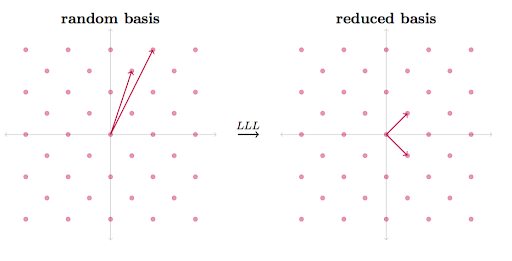
\includegraphics[width=0.8\linewidth,height=6cm]{pictures/basis_reduction.png}
\caption{Σχηματική απεικόνιση της αναγωγής βάσης κατά LLL, όπου διακρίνεται τόσο η ορθογωνιότητα των διανυσμάτων, όσο και η συρρίκνωσή τους.}
\label{fig:LLL}       
\end{figure}

Ιδιαίτερη σημασία για τη χρήση του αλγορίθμου LLL έχει το παρακάτω θεώρημα, βάση του οποίου ο αλγόριθμος επιτυγχάνει πολυωνυμική σύγκλιση. 

\begin{theorem}: 
Για μία n-διάστατη βάση $B = \{\bm b_1, ..., \bm b_n \} $, ο αλγόριθμος LLL με $ \delta = 3/4 $ έχει πολυωνιμική πολυπλοκότητα ως προς το μήκος των διανυσμάτων της βάσης και συγκεκριμένα: $ O(n^4log_2Μ) $, όπου $ Μ = \max_i(\| \bm b_i\|^2)$.
\end{theorem}
\emph{Απόδειξη.} \cite{journals/siamcomp/NguyenS09}